\documentclass[11pt]{article}
\usepackage{fullpage,amsthm,amsfonts,amssymb,epsfig,amsmath,times,amsthm,enumitem,mathtools,graphicx}

\newtheorem{theorem}{Theorem}
\newtheorem{claim}[theorem]{Claim}
\DeclarePairedDelimiter\ceil{\lceil}{\rceil}
\DeclarePairedDelimiter\floor{\lfloor}{\rfloor}
\graphicspath{{imgs/}}

\begin{document}

\begin{center}
{\bf\Large CMPS 142 --- Spring Quarter 2017 --  Homework 1}\\
{\bf Christopher Hsiao - chhsiao@ucsc.edu - 1398305}\\
{\bf Aidan Gadberry - agadberr@ucsc.edu}
\end{center}

\section*{2 - Linear Regression in Weka}
\textbf{a.)} Root Mean Squared Error: 0.1897\\
\textbf{b.)} For $x = [3, 3, 5]$, our model $-0.1343(x_1) + 1.8477(x_2) + -0.8966(x_3) + 4.3608 = 5.018$\\
\textbf{c.)}
\begin{align}
w = [1, 1, 1, 1] \ \ \eta = 0.1 \\ 
x^{(1)} = [1, 3, 9, 2] \ \ y^{(1)} = 19 \\
x^{(2)} = [1, 6, 9, 1] \ \ y^{(2)} = 19 \\
w_j = w_j + \eta(y^{(i)} - w^Tx^{(i)})x^{(i)}_j
\end{align}
\begin{center}
And using the update rule $(4)$ for each feature $j$ in instance $i$.
\end{center}

Step 1: 
\begin{align*}
w_0 = 1 + 0.1(19 - 15)1 = 1.4\\
w_1 = 1 + 0.1(19 - 15)3 = 2.2\\
w_2 = 1 + 0.1(19 - 15)9 = 4.6\\
w_3 = 1 + 0.1(19 - 15)2 = 1.8\\
w = [1.4, 2.2, 4.6, 1.8]
\end{align*}

Step 2:
\begin{align*}
w_0 = 1.4 + 0.1(19 - 57.8)1 = -2.48\\
w_1 = 2.2 + 0.1(19 - 57.8)6 = -21.08\\
w_2 = 4.6 + 0.1(19 - 57.8)9 = -30.32\\
w_3 = 1.8 + 0.1(19 - 59.6)1= -2.08\\
w = [-2.48, -21.08, -30.32, -2.08]
\end{align*}

\textbf{d.)}
\begin{equation}
\text{Closed Form: } w = (X^TX)^{-1}X^Ty
\end{equation}
\[X =
\begin{bmatrix}
1, 3, 9, 2\\
1, 6, 9, 1\\
1, 7, 7, 7\\
1, 8, 6, 4\\
1, 1, 0, 8
\end{bmatrix}
\ \ y =
\begin{bmatrix}
19\\
19\\
10\\
11\\
-3
\end{bmatrix}
\ \ X^T = 
\begin{bmatrix}
1, 1, 1, 1, 1\\
3, 6, 7, 8, 1\\
9, 9, 7, 6, 0\\
2, 1, 7, 4, 8
\end{bmatrix}
\]
\begin{center}
\pagebreak
Now, we calculate $X^TX \ \text{and} \ X^Ty$
\end{center}
\[X^TX = 
\begin{bmatrix}
5, \ 25, \ 31, \ \ 22\\
25, 159, 178, 101\\
31, 178, 247, 100\\
22, 101, 100, 134
\end{bmatrix}
\ \ x^Ty = 
\begin{bmatrix}
56\\
326\\
478\\
147
\end{bmatrix}
\]
\begin{center}
Putting it all together, we get:
\end{center}
\[w= 
\begin{bmatrix}
4.361\\
-0.134\\
1.848\\
-0.897
\end{bmatrix}\]
\textbf{e.)}
During Batch Gradient Descent, the order with which the rows (examples) are seen doesn't matter, since every example will be seen every iteration anyway. Reordering the parameters would definitely impact the model with respect to the features they're representing. For example, a quadratic function will have different weights associated with the features, but features would have different degrees.

\section*{Experiments on Linear Regression\\}
\textbf{(a)} Closed form solution for Linear Regression\\
\textbf{Training Set Error\\}
$k = 10$: t1 error: 0.00251713330282 t2 error:0.000288814927052\\
$k = 100$: t1 error: 0.000366640819671 t2 error:0.00177654927121\\
$k = 1000$: t1 error: 3.03489776154e-05 t2 error:0.000749918991201\\
$k = 10000$: t1 error: 0.00016024779446 t2 error:0.000143860751203\\

\textbf{Test Set Error\\}
$k = 10$: t1 error: -0.0103056950245 t2 error:-0.000254256403195\\
$k = 100$: t1 error: -0.000472129192032 t2 error:-0.00248682014886\\
$k = 1000$: t1 error: 0.00101928449978 t2 error:-0.000520347427673\\
$k = 10000$: t1 error: 0.00016024779446 t2 error:0.000143860751203\\

By calculating the closed form solution to the problem, we found that the closed form does a pretty good job at estimating $\theta$, with fairly small error. As $k$ increases, the accuracy of the algorithm increases with $k$ as well.

\textbf{(b)}
\begin{center}
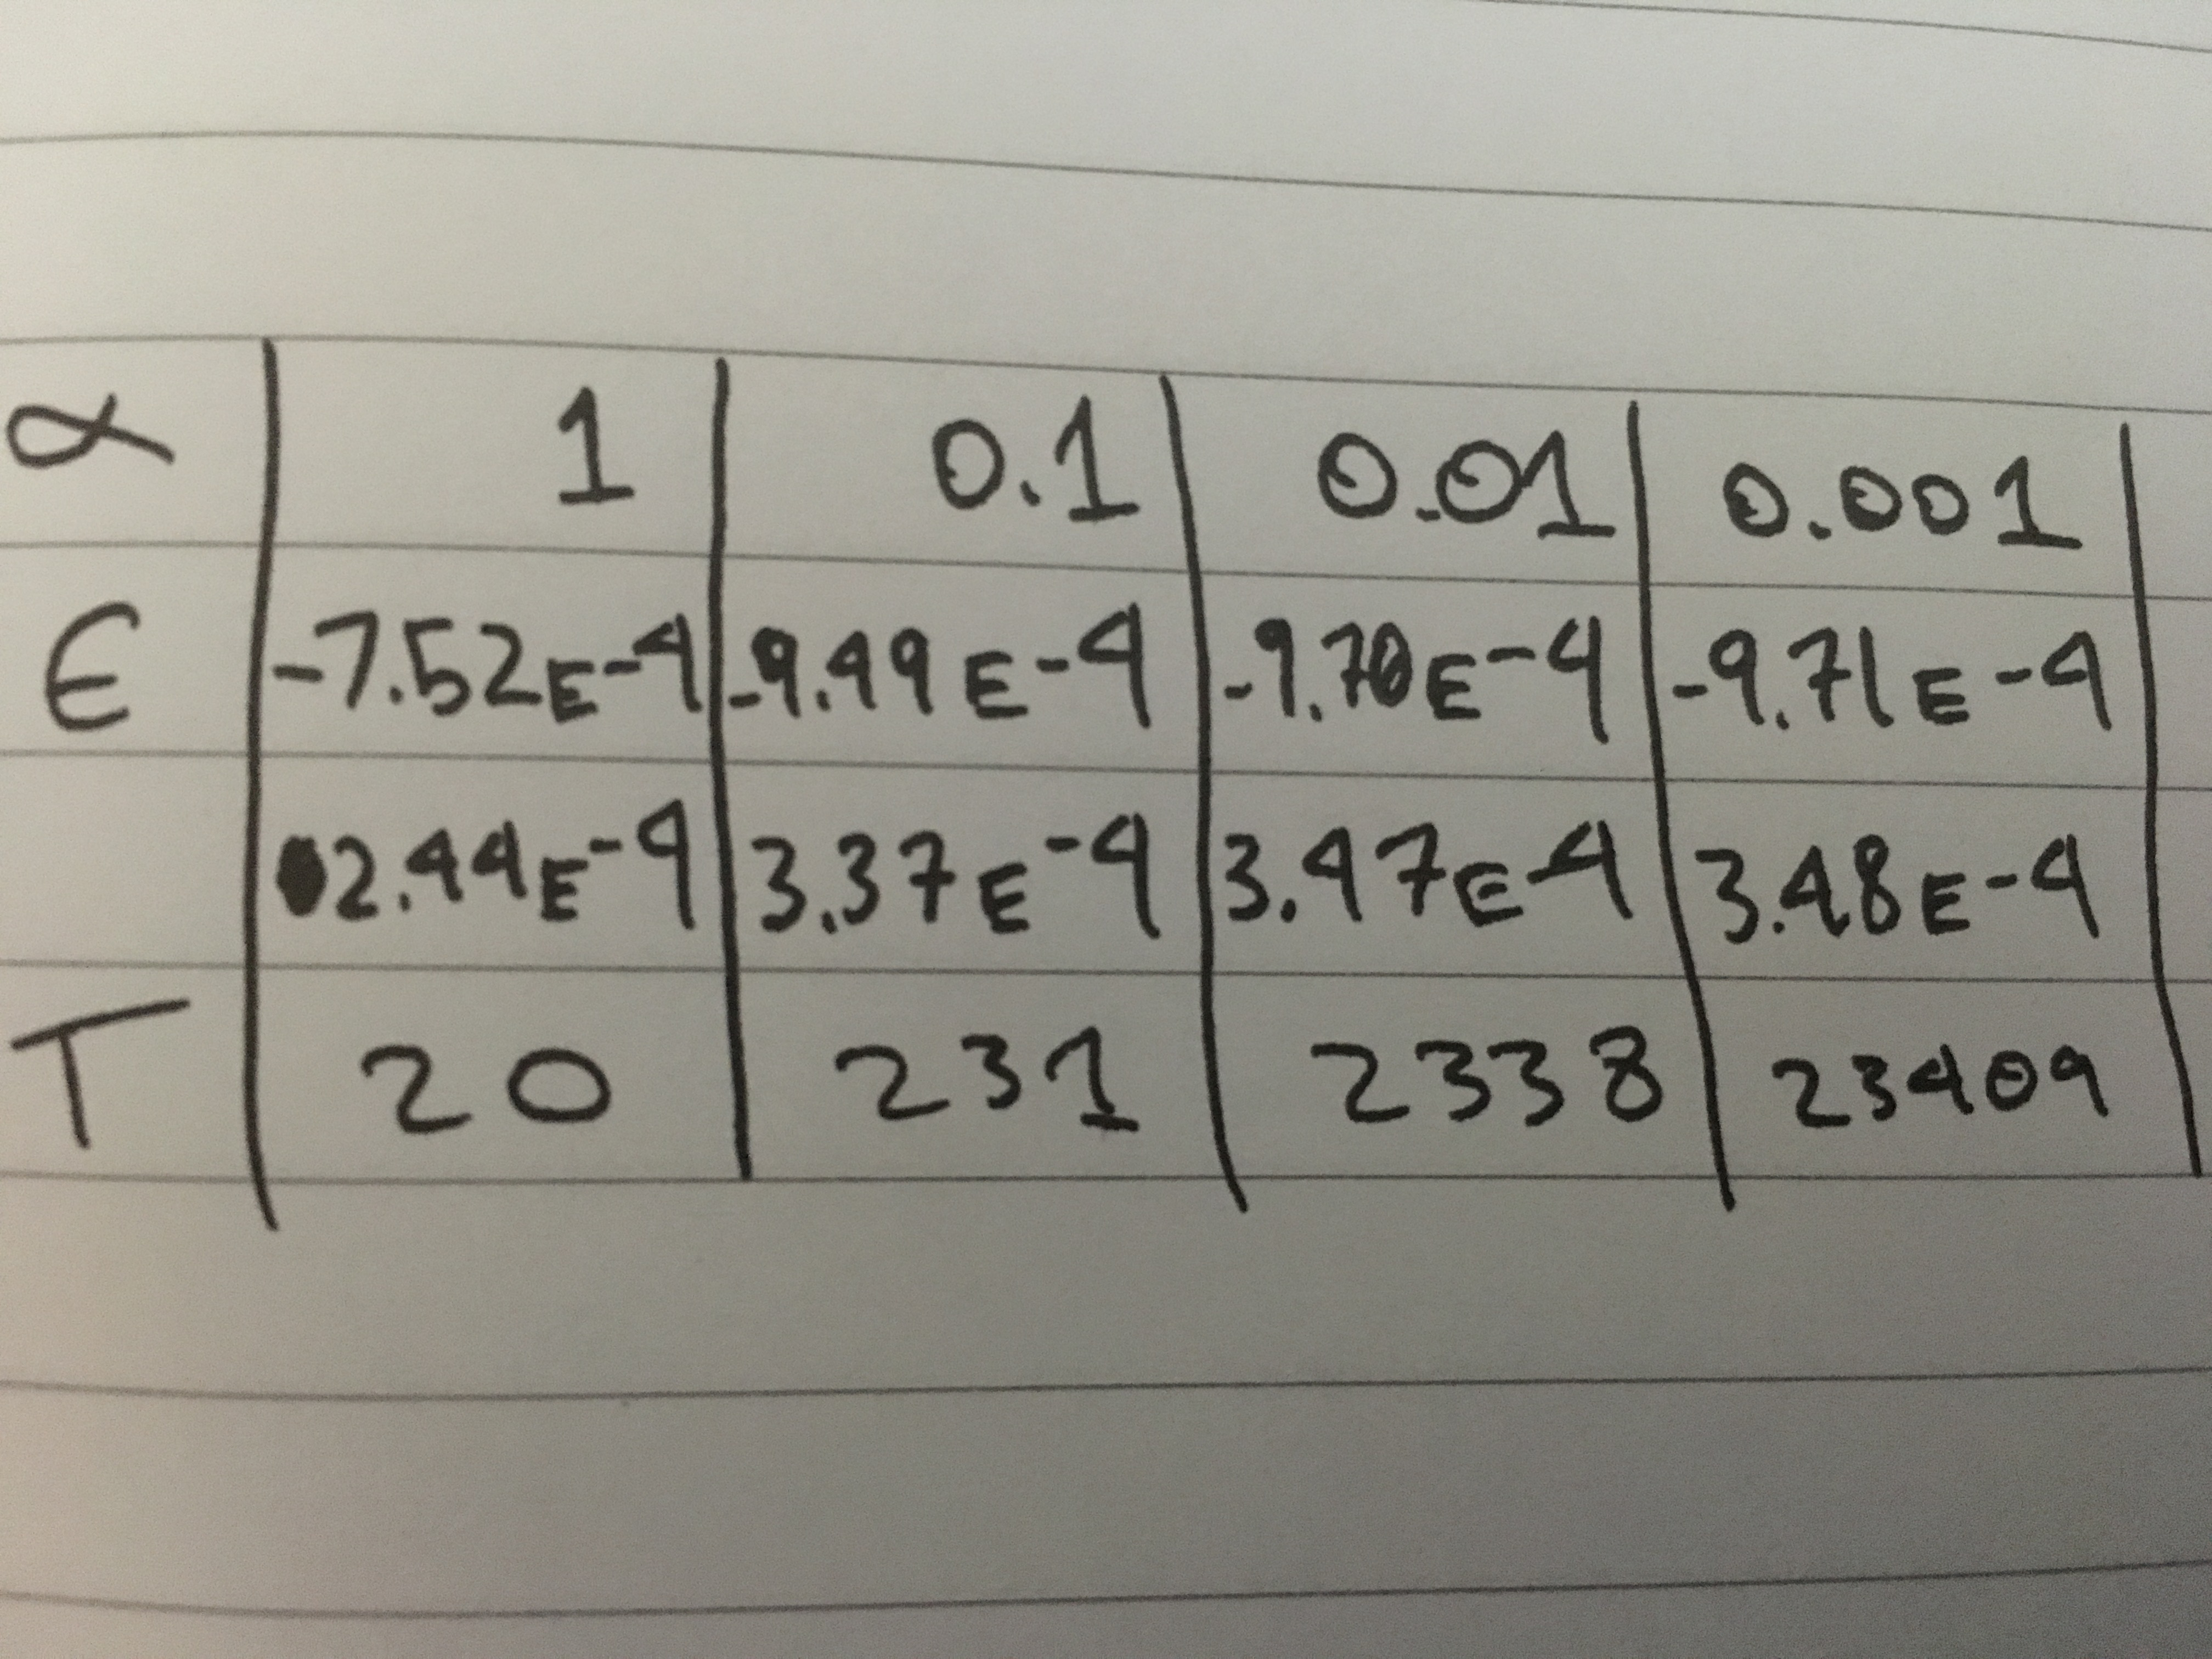
\includegraphics[width=10cm,height=10cm,keepaspectratio]{3b} \end{center}

Clearly, since we have a smaller learning rate as we progress, the number of iterations required to reach the minima will increase by a factor of 10 (as we vary our $\alpha$ by 10). The error actually plateaus in comparison with the closed form solution, primarily because of the fact that the closed form solution doesn't reach the same levels of accuracy as the smaller learning rates enable when randomly selecting from the data sets. \\
\\
\textbf{(c)} Sophisticated Step Sizes:\\
This algorithm takes 22193 iterations. The $\epsilon$ difference in this hypothesis and the closed solution is: $[-1.10E-4, 5.37E-4]$

\section*{Titanic}
In order to predict the odds of survival of a passenger with 100\% accuracy, one can simply look up the logs of passengers on the Titanic, and simply resort to table look up.\\

This implies that Machine learning is not always the best way to go about approaching a problem first, and that there may be underlying structure to your problem that you're simply not noticing.



\end{document}